%!TEX root = ../main.tex

\section{Постановка задачи}

\begin{frame}{Одномерная задача}
\vspace{-0.3cm}
\begin{itemize}
	\item Область $\clOmega = [0, W]_x \times [0, H]_y \times I_z$ в форме параллелепипеда
	\item $\phi(\vx, 0) = \phi_0(\vx) = \phi_0(x)$, $\epsilon_0(\vx) = \epsilon_0(x)$ не зависят от $y$ и $z$
	\item $\Phi|_{y = 0} = \Phi^- \in \mathbb{R}$, $\Phi|_{y = h} = \Phi^+ \in \mathbb{R}$
\end{itemize}
Подробнее в работе \cite{ponomarev_stability}. \\[0.3cm]
Решением является функция электрического потенциала
\begin{columns}
\column{0.65\textwidth}
	\vspace{-1cm}
	$$\Phi(\vx, t) = \Phi^- \hm + \cfrac{y}{h}(\Phi^+ - \Phi^-).$$
\column{0.35\textwidth}
	\begin{figure}
		\vspace*{-2.3cm}
		\hspace*{0.5cm}
		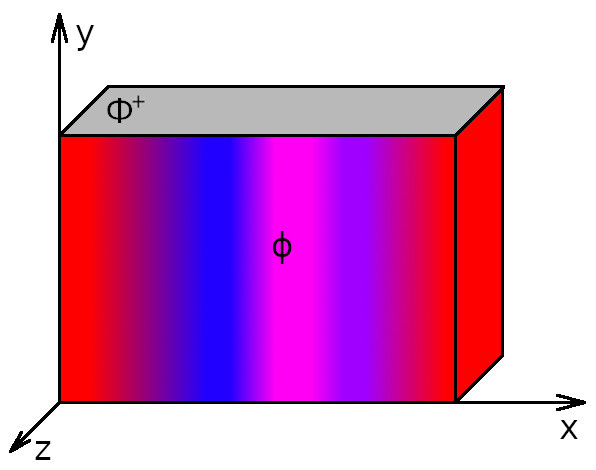
\includegraphics[width=0.85\textwidth]{figures/one_dim_problem.jpg}
	\end{figure}
\end{columns}
\vspace{-0.4cm}
Тогда уравнение на $\phi$ принимает вид
\begin{block}{}
	$$\cfrac{1}{m} \partt{\phi} = \half K_\Phi^2 \epsilon'(\phi) + \cfrac{\Gamma}{l^2} f'(\phi) + \half \Gamma \partxx{\phi}$$
\end{block}
$K_\Phi = \cfrac{\Phi^+ - \Phi^-}{h} = \norm{\nabla \Phi}$. Будем считать $\epsilon_0 = \Const$.
\end{frame}


\section{Теоретический анализ}

\begin{frame}{Анализ положений равновесия}
\begin{itemize}
	\item Канал пробоя может развиваться из малых возмущений свойств неповрежденной среды. Выясним условия развития.
	\item Рассмотрим положения равновесия вида $\phi(x, t) \equiv C$. Положению равновесия соответствует ноль $C$ функции
\end{itemize}
$$\chi(\phi) = \half K_\Phi^2 \epsilon'(\phi) + \cfrac{\Gamma}{l^2} f'(\phi).$$
\vspace{-0.5cm}
\begin{itemize}
	\item Исследуем положения равновесия на устойчивость спектральным методом: к $\phi \equiv C$ прибавим возмущение $\delta \phi = e^{\alpha t} \sin(\omega x)$, линеаризуем уравнение на $\delta \phi$.
	\item $\chi(\phi)$ возрастает в $C \Longrightarrow$ равновесие неустойчиво; $\chi(\phi)$ убывает в $C \Longrightarrow$ равновесие устойчиво.
\end{itemize}
\end{frame}


\begin{frame}{Анализ положений равновесия}
\vspace{-0.9cm}
\begin{columns}
\column{0.3\textwidth}
	\begin{center}
		<<Слабое>> напряжение
	\end{center}
	\vspace{-0.2cm}
	$$0 \leqslant \cfrac{K_\Phi^2 l^2 \epsilon_0}{2 \Gamma} < \delta^2$$
	\vspace{-0.7cm}
	\begin{figure}
		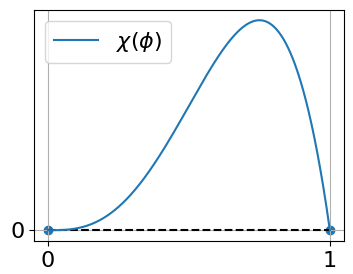
\includegraphics[width=\textwidth]{figures/equilibriums_case_1.png}
	\end{figure}
\column{0.3\textwidth}
	\begin{center}
		<<Среднее>> напряжение
	\end{center}
	\vspace{-0.2cm}
	$$\delta^2 < \cfrac{K_\Phi^2 l^2 \epsilon_0}{2 \Gamma} < (1 + \delta)^2$$
	\vspace{-0.7cm}
	\begin{figure}
		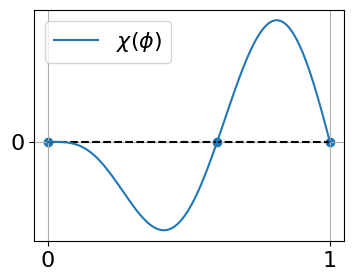
\includegraphics[width=\textwidth]{figures/equilibriums_case_2.png}
	\end{figure}
\column{0.3\textwidth}
	\begin{center}
		<<Сильное>> напряжение
	\end{center}
	\vspace{-0.2cm}
	$$(1 + \delta)^2 < \cfrac{K_\Phi^2 l^2 \epsilon_0}{2 \Gamma}$$
	\vspace{-0.7cm}
	\begin{figure}
		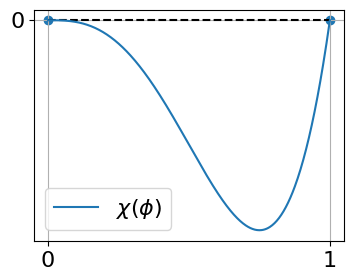
\includegraphics[width=\textwidth]{figures/equilibriums_case_3.png}
	\end{figure}
\end{columns}
\begin{columns}
\column{0.3\textwidth}
	\hspace{0.5cm}
	$\phi \equiv 0$ неустойчивое \\
	\hspace{0.5cm}
	$\phi \equiv 1$ устойчивое
\column{0.3\textwidth}
	\hspace{0.5cm}
	$\phi \equiv 0$ устойчивое \\
	\hspace{0.5cm}
	$\phi \equiv С_3$ неустойчивое \\
	\hspace{0.5cm}
	$\phi \equiv 1$ устойчивое
\column{0.3\textwidth}
	\hspace{0.5cm}
	$\phi \equiv 0$ устойчивое \\
	\hspace{0.5cm}
	$\phi \equiv 1$ неустойчивое
\end{columns}
\end{frame}


\section{Численный анализ}

\begin{frame}{Разностная схема}
\begin{block}{Разностная задача}
	$$\cfrac{1}{m} \cfrac{\phi_i^{j + 1} - \phi_i^j}{\tau} = \half K_\phi^2 \epsilon'(\phi_i^j) + \cfrac{\Gamma}{l^2} f'(\phi_i^j) + \cfrac{\Gamma}{2} \cfrac{\phi_{i + 1}^j - 2 \phi_i^j + \phi_{i - 1}^j}{h^2}$$
	$$\phi_i^0 = \phi_0(ih); \quad \phi_0^j = \phi_l(j \tau); \quad \phi_n^j = \phi_r(j \tau)$$
	Сетка регулярная; $\tau$ -- шаг по времени, $h$ -- шаг по пространству.
\end{block}
Явная разностная схема первого порядка по времени, второго -- по пространству.
\end{frame}


\begin{frame}{Оценка устойчивости}
\begin{itemize}
	\item Рассмотрим возмущенное решение $\phi_i^j + \delta_i^j$. Линеаризуем уравнение на возмущение $\delta_i^j$ в точке $\phi_i^j = P$:
\end{itemize}
$$\delta_i^{j + 1} = \delta_i^j + m \tau \left( \half K_\Phi^2 \epsilon''(P) \delta_i^j + \cfrac{\Gamma}{l^2} f''(P) \delta_i^j + \cfrac{\Gamma}{2} \cfrac{\delta_{i + 1}^j - 2 \delta_i^j + \delta_{i - 1}^j}{h^2} \right).$$
\begin{itemize}
	\item Применим спектральный признак устойчивости:
\end{itemize}
$$1 > | \lambda(\theta) | = \left| 1 + m \tau \left( \half K_\Phi^2 \epsilon''(P) + \cfrac{\Gamma}{l^2} f''(P) - \cfrac{2 \Gamma}{h^2} \sin^2 \cfrac{\theta}{2} \right) \right|.$$
\begin{itemize}
	\item Исследуем вблизи $P = 0$.
\end{itemize}
\end{frame}


\begin{frame}{Оценка устойчивости}
\begin{block}{Условие устойчивости}
	$$\tau \leqslant \cfrac{1}{2 m} \left( \cfrac{K_\Phi^2 \epsilon_0}{\delta^{5/3}} + \cfrac{\Gamma}{h^2} \right)^{-1}$$
\end{block}
\begin{block}{Упрощенное условие устойчивости}
	$$\tau \leqslant \cfrac{1}{4 m} \min \left(\cfrac{\delta^{5/3}}{K_\Phi^2 \epsilon_0}, \; \cfrac{h^2}{\Gamma} \right)$$
\end{block}
\end{frame}


\begin{frame}{Вычисления: типичное решение}
\vspace{-0.4cm}
\begin{columns}
\column{0.88\textwidth}
\begin{figure}
	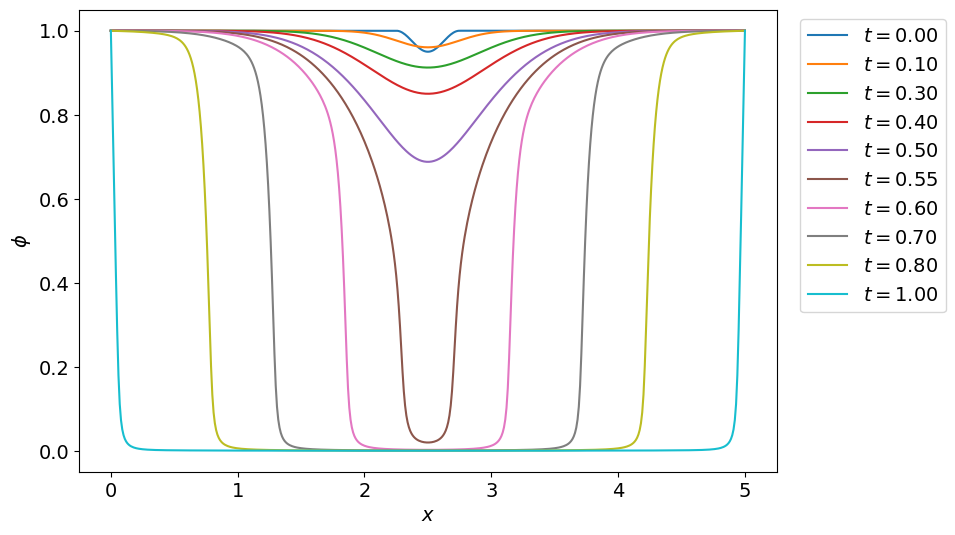
\includegraphics[width=\textwidth]{figures/typical_solution.png}
\end{figure}
\column{0.12\textwidth}
\hfill \\
\vspace{3.5cm}
\hspace{-2.5cm}
Узлов по измерениям: \\
\hspace{-2.5cm}
$N_x = 10^3$, $N_t = 10^5$
\end{columns}
\end{frame}


\begin{frame}{Вычисления: проверка устойчивости}
\vspace{-0.4cm}
\begin{columns}
\column{0.7\textwidth}
\begin{figure}
	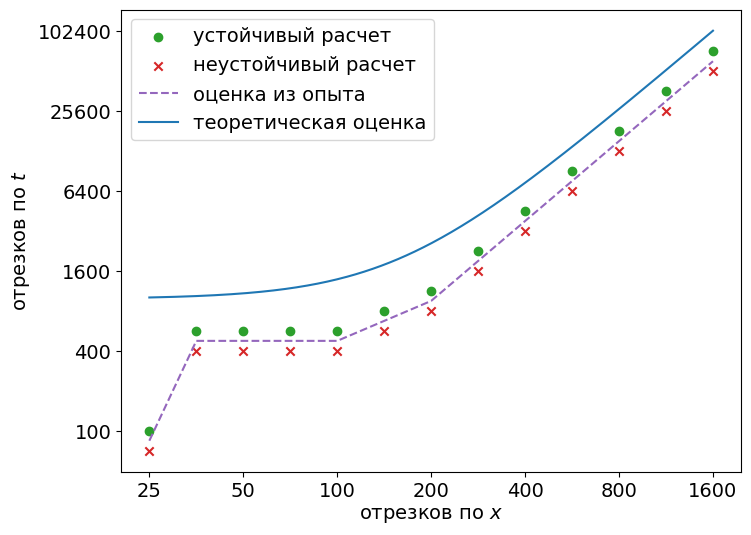
\includegraphics[width=\textwidth]{figures/stability_bounds.png}
\end{figure}
\column{0.3\textwidth}
Условие устойчивости:
$$\tau \leqslant \cfrac{1}{2m} \left( \cfrac{K_\Phi^2 \epsilon_0}{\delta^{5/3}} +
\cfrac{\Gamma}{h^2} \right)^{-1}$$
\end{columns}
\end{frame}


\begin{frame}{Вычисления: проверка сходимости}
\vspace{-0.3cm}
\begin{figure}
	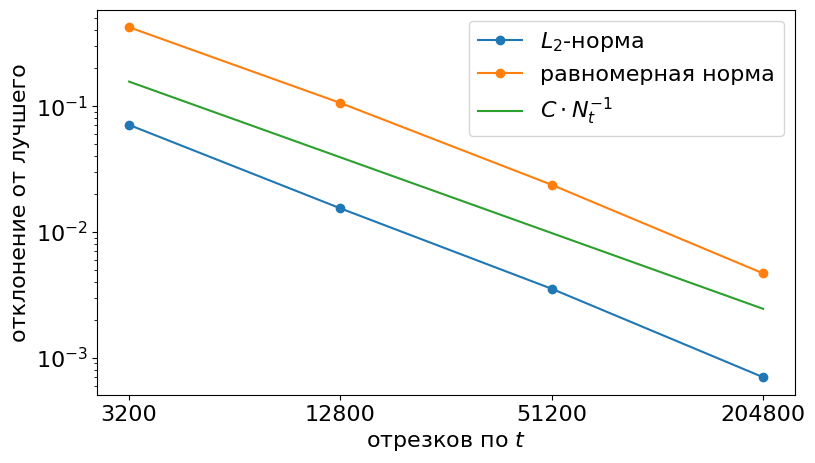
\includegraphics[width=0.58\textwidth]{figures/convergence_connected.png}
\end{figure}
\vspace{-0.6cm}
\begin{center}
	Здесь, согласно оценке устойчивости, $\tau = \cfrac{h^2}{4m \Gamma}$
\end{center}
\end{frame}


\begin{frame}{Вычисления: положения равновесия}
\vspace{-0.4cm}
\begin{center}
	$(1 + \delta)^2 < \cfrac{K_\Phi^2 l^2 \epsilon_0}{2 \Gamma}$ -- <<сильное>> напряжение
\end{center}
\vspace{-0.4cm}
\begin{columns}
\column{0.5\textwidth}
\begin{figure}
	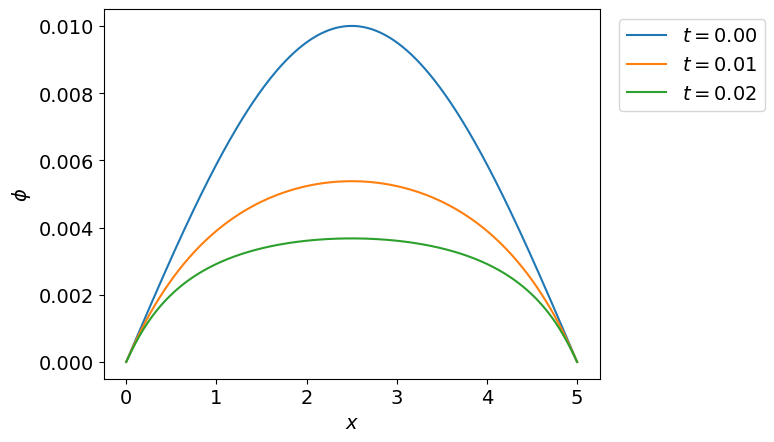
\includegraphics[width=\textwidth]{figures/equilibrium_3_0.png}
\end{figure}
\vspace{-0.8cm}
\begin{center}
	$\phi \equiv 0$, устойчивое
\end{center}
\column{0.5\textwidth}
\begin{figure}
	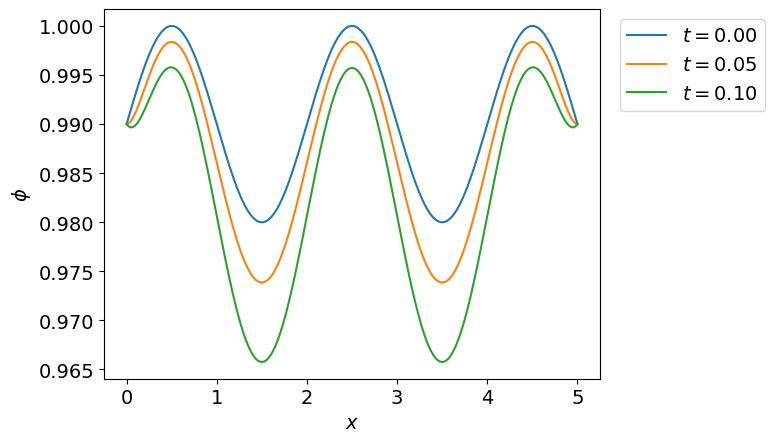
\includegraphics[width=\textwidth]{figures/equilibrium_3_1.png}
\end{figure}
\vspace{-0.8cm}
\begin{center}
	$\phi \equiv 1$, неустойчивое
\end{center}
\end{columns}
\end{frame}


\begin{frame}{Свободная энергия}
\vspace{-0.5cm}
$$\Pi(t) = \int\limits_\Omega \pi(x, t) dx$$
$$\pi = -\half \epsilon[\phi] \gradscalsq{\Phi} + \Gamma \left( \cfrac{1 - f(\phi)}{l^2} + \cfrac{1}{4} \gradscalsq{\phi} \right)$$
\begin{itemize}
	\item Уравнения \eqref{equation_potential}, \eqref{equation_phase} выведены так, что система в ходе эволюции стремится в состояние с как можно меньшей полной свободной энергией $\Pi$.
	\item Необходимо, чтобы указанное свойство выполнялось при моделировании.
\end{itemize}
\end{frame}


\begin{frame}{Вычисления: свободная энергия}
\vspace{-0.6cm}
\begin{figure}
	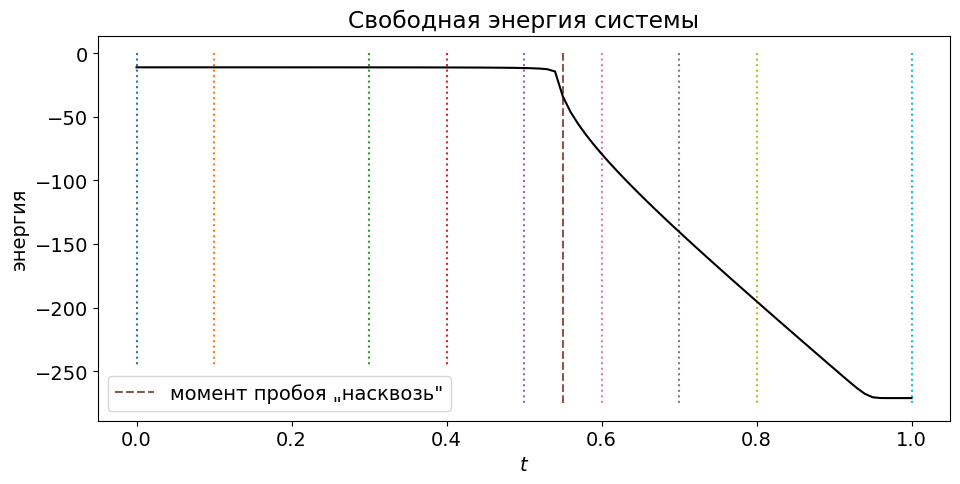
\includegraphics[width=0.88\textwidth]{figures/energy_total.png}
\end{figure}
\end{frame}